\section{Justificaci\'on del Proyecto}\label{sec:justificacion}

A medida que crece el requerimiento de ancho de banda de los usuarios
en internet, las empresas proveedoras del servicio deben utilizar más
y mejores tecnologías extensibles y flexibles que posibiliten este
proceso.

En esta sección se expondrán los detalles de la justificación del
proyecto, es decir, se mostrarán los aspectos cuantitativos y
cualitativos que permitirán convencerse de que el proyecto es
conveniente.

\subsection{Aspectos cuantitativos}
\label{sec:cuantitativos}

Los aspectos que permiten visualizar en forma contable la conveniencia
del proyecto se deben traducir a términos monetarios. El objetivo es
que la empresa pueda ver de forma clara el contraste entre tener una
red de fibra oscura e instalar una red de fibra activa.

Las redes fotónicas ``oscuras'', es decir, sin ningún tipo de
multiplexación o control de las señales al momento de introducirlas en
la fibra, no son adecuadas para montar redes modernas que requieran
grandes anchos de banda. Este es el caso de los enlaces entre 
datacenters, donde el volumen y la importancia de los datos que fluyen
hacia y desde sus nodos deben cumplir con un tiempo de acceso cada vez
más rápido y por un número creciente de usuarios.

En efecto, lo correcto para notar esta diferencia sustancial en este
contexto es considerar la capacidad de un cable de fibra óptica con y
sin multiplexación en frecuencia. Si cada cable de G.652.D tiene 96
fibras en su interior, entonces se pueden conectar un total de 96
servicios por cada cable. Si se considera un canal de ancho 50 GHz y
protocolos Ethernet de 100 GB/s\footnote{Cerca del tope de la
  tecnología existente al momento de elaborar este informe.}, la
capacidad total de una fibra oscura es de 9.6 TB/s. Considerando la
misma configuración de protocolos en una red \emph{DWDM}, el cable
óptico permite el transporte de 80 veces este valor, es decir, cerca
de 768 TB/s, lo que representa una disminución de costo de instalación
de tendido. Para poder alcanzar este ancho de banda de hubiera
necesitado instalar 80 cables de fibra óptica adicionales en cada uno
de los tramos que en total suman 399 Km.

El análisis anterior supone que los tendidos ya se encuentran
empalmados y operando correctamente con cada uno de los servicios
requeridos. Sin embargo, un corte de alguna fibra significaría que
dejarían de operar algunos de los puntos de red, mientras que un corte
en el cable completo significaría el apagado de 80 puntos de red a la
vez, algo que seguramente afectaría el \emph{SLA} y con ello muchos de
los contratos con clientes.

A continuación se muestra una simulación de los costos de romper el
\textsf{SLA} con clientes: si se supone que cada puerto operativo
tiene asociado contratos que suman USD
\$1.000.000\footnote{Aproximación burda; es probable que el orden de
  magnitud de este valor haya sido subestimado.} en ingresos anuales
para Entel, la ruptura de un cable significaría perder alrededor de 
USD \$30.000.000 de ingresos anuales en el caso que las empresas 
involucradas renuncien al caerse el servicio.

Una fibra activa con sistemas \emph{WSS} y \emph{WSON} para
restablecer las rutas automáticamente significarían un costo inicial 
como el mencionado en la sección \ref{sec:capex}, pero el
costo de romper contratos por \emph{SLA} se ahorraría.

Un análisis cuantitativo menos dramático tiene que ver con el costo de
la mantención de los equipos. Mantener equipos de fibra oscura
requeriría recurrentemente empalmar fibras, tender nuevos cables e
instalar mayor cantidad de \emph{ODFs}. Ello elevaría el costo por mano
de obra pues las obras durarían mucho más. Además, la cantidad de
conexiones que se crearían sería difícil de predecir, haciendo que la 
probabilidad de cometer errores que terminen afectando el \emph{SLA} 
de los clientes aumente considerablemente.

Los puntos cuantitativos negativos de instalar un sistema \emph{DWDM}
que reemplace al tendido de fibra oscura se pueden observar desde el
punto de vista técnico. Equipos más complejos requerirán mano de obra
especializada y aumento en costo de energía. Sin embargo, estos costos
(ver secciones \ref{sec:capex} y \ref{sec:opex}) son marginales con 
respecto al riesgo de afectar al \emph{SLA}.

En síntesis, la comparación es claramente favorable para una red 
iluminada, pues los riesgos que se toman al violar el \emph{SLA} de los
clientes es mayor a cualquier inversión que se pueda realizar. Por ello, 
se recomienda invertir en \emph{iluminar} la red de fibra óptica.

\subsection{Aspectos cualitativos}
\label{sec:cualitativos}

Los aspectos argumentables de forma no contable que permiten
establecer la conveniencia del proyecto son los que se muestran en
esta sección.

Como muestra la figura \ref{fig:aumento_bw}, el crecimiento de ancho
de banda a nivel global está en aumento constante. Se espera que este
crecimiento no se detenga nunca, ya que a medida que el ser humano
tiene acceso a más velocidad, sus necesidades y exigencias tecnológicas
aumentan.

\begin{figure}[H]
  \centering
  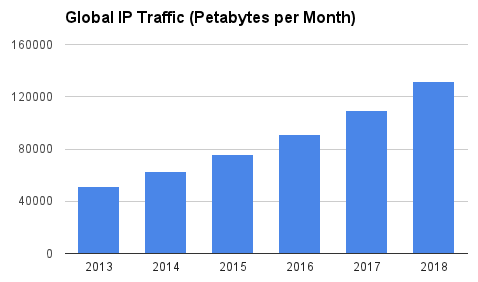
\includegraphics[width=0.75\textwidth]{Imagenes/iptrafficchart.png}
  \caption{Tendencia en el aumento del ancho de banda a nivel mundial
    según un estudio de Cisco de 2014.\cite{ciscoiptraffic}}
  \label{fig:aumento_bw}
\end{figure}

\emph{DWDM} es una tecnología en esencia modular y escalable. Todos
los proveedores de esta tecnología ofrecen actualizaciones en forma de
módulos para poder reemplazar los equipos obsoletos con versiones
nuevas o bien para expandir y mejorar el soporte de las tecnologías
tradicionales a más tendidos.

La incursión de los \emph{ROADM} hacia un sistema programable con
variedad de filtros integrados y con manejo de eventos, como lo son
los dispositivos \emph{WSS}, ha significado que la flexibilidad de
\emph{DWDM} sea mayor que nunca. Por otro lado, los precios de estos
dispositivos han disminuido de forma considerable en los últimos años,
haciéndose populares y soportados globalmente.

Algunos de los servicios más pintorescos que permiten implementar los
data centers en el mundo son los que se muestran en la figura
\ref{fig:servicios}.

\begin{figure}[H]
  \centering
  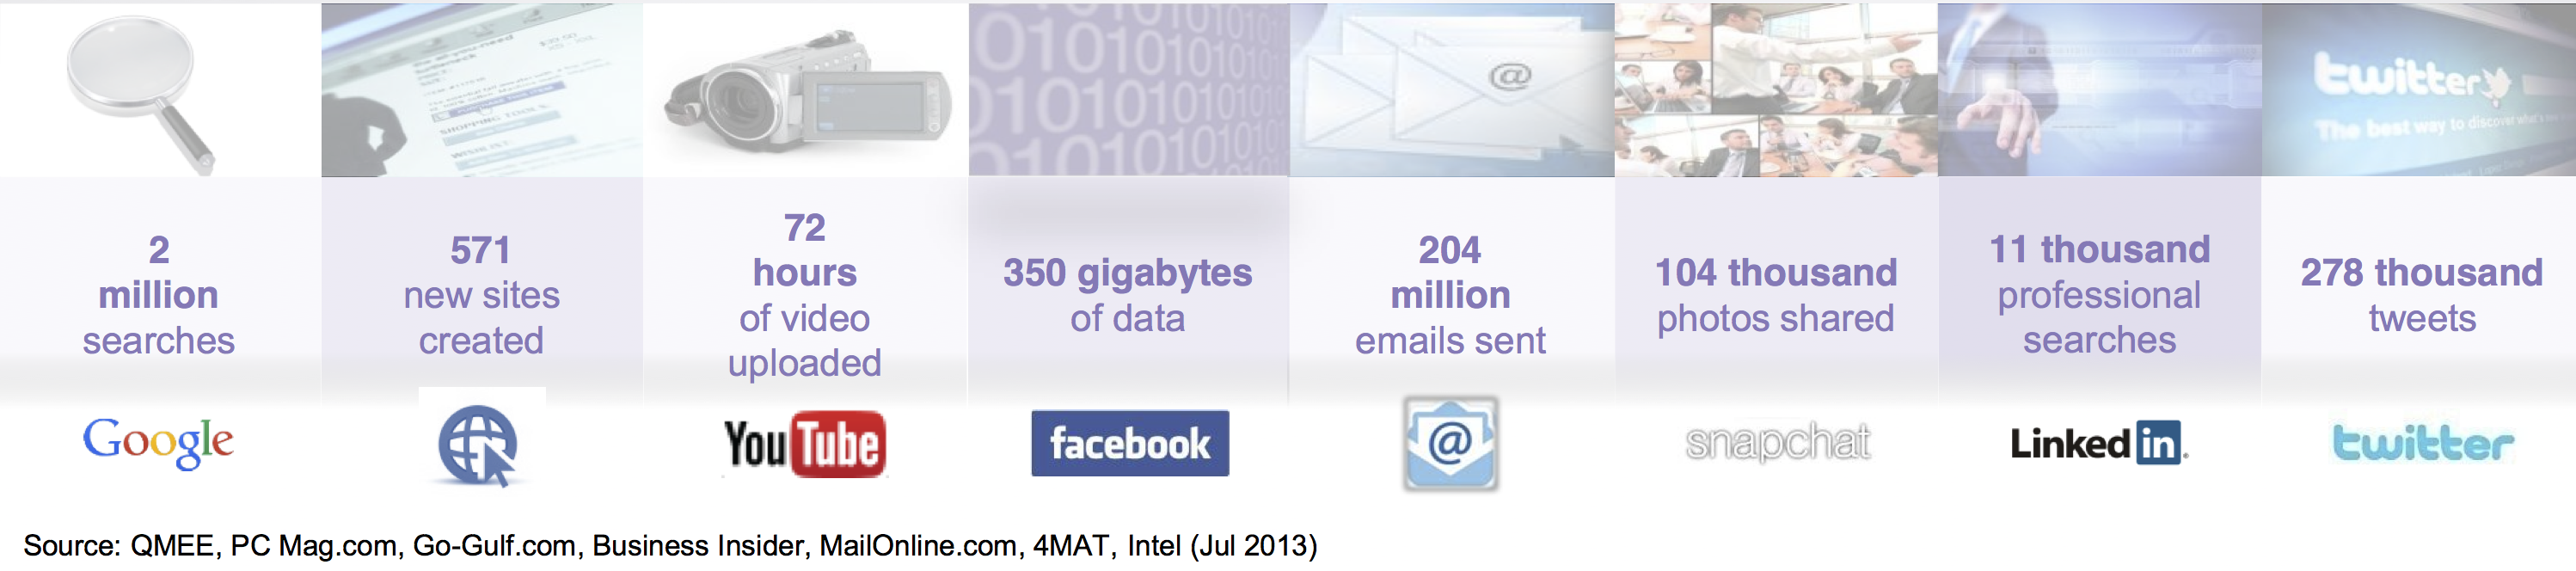
\includegraphics[width=15cm]{Imagenes/servicios.png}
  \caption{Servicios en los que participan data centers que ocupan una
    muy alta y creciente cantidad de capacidad instalada en las
    redes. Datos de julio de 2013 provenientes de: QMEE, PC Mag.com,
    Go-Gulf.com, Business Insider, MailOnline.com, 4MAT e Intel.}
  \label{fig:servicios}
\end{figure}

Los servicios mostrados en la figura \ref{fig:servicios} son algunos
de los más famosos en la Web a la fecha. Por otro lado, existen 
ambientes de alto tráfico en el ámbito de los observatorios espaciales
y grupos científicos, que deben manejar del orden de petabytes de
información por día. Estos volúmenes de información sólo pueden ser
manejados en la actualidad por data centers. Sin embargo, el
transporte de estos datos es uno de los cuellos de botella más
críticos del sistema de almacenamiento de información y de las nuevas
tecnologías en el mundo en general.

Este aumento en el flujo de información requiere de redes que se puedan
instalar rápidamente, sin realizar inversiones demasiado grandes y que
tengan la posibilidad de escalar fácilmente en el tiempo. En este
sentido, el argumento nuevamente favorece migrar a \emph{DWDM} en vez
de mantener la fibra oscura. 

En definitiva, los avances, la estandarización y la disminución de
precios que han experimentado este tipo de tecnologías son los
factores más importantes que permiten justificar el proyecto de forma
cualitativa.
